\chapter{Construcción del catálogo de Datasheets de APIs de correo}
\label{cap:catalogo}

Este capítulo presenta el método con el que se construye el catálogo de
Datasheets de APIs de correo electrónico (la contribución C-01 de la
Sección~\ref{sec:introduccion:contribuciones}) y su calibración sobre un
piloto real. Se organiza en cinco piezas. El criterio de selección del
dominio. El ciclo de construcción por API. Las reglas de trazabilidad y
confianza que hacen revisable cada dato. La escalera de validación que
convierte inferencias en evidencia. Y el marco de conformidad y evolución
del esquema.
Le sigue el piloto (Postmark) con los hallazgos que validan el método y anticipan la evolución del esquema (contribución C-02).
Esa evolución no se formula aquí: se pospone al cierre del catálogo, conforme al criterio de promoción de la Sección~\ref{sec:propuesta:conformidad}, y ocupa el Capítulo~\ref{cap:evolucion}.
El capítulo se cierra con la respuesta a la RQ1 (Sección~\ref{sec:propuesta:respuesta}).

\section{Criterio de selección del dominio}
\label{sec:propuesta:seleccion}

El dominio del catálogo son las APIs de correo transaccional.
Postmark, una de las ocho, define el correo transaccional como un mensaje individual que el destinatario espera recibir y que suele desencadenar el propio usuario \citep{postmarktransaccional}.
Pone como ejemplos el restablecimiento de contraseña, el recibo de compra o el aviso de pago fallido.
Excluye el correo con el mismo contenido para muchos destinatarios que no desencadena ningún evento, al que llama de \textit{marketing}.
Una API de correo transaccional es la interfaz con la que una aplicación entrega esos mensajes a través del proveedor.
El producto de \textit{marketing} que varios proveedores venden en la misma cuenta queda fuera (Sección~\ref{sec:propuesta:criterios}).
Hasta dónde valen los resultados fuera de este dominio lo discute la Sección~\ref{sec:conclusiones:externa}.

El conjunto de APIs analizadas se determina con el criterio fijado en el encargo del trabajo, que combina tres fuentes de inclusión.
La selección se completó el 1 de septiembre de 2026 con la tercera fuente, una consulta a un modelo de lenguaje con cinco criterios fijados antes de hacerla.
El Anexo~\ref{anx:uso-ia} registra la fecha, el modelo, el prompt con sus criterios y la respuesta íntegra de la consulta, y señala lo que no consta.
Con ese registro un tercero puede repetir la consulta con el mismo prompt y contrastar lo que obtenga con lo que recoge el anexo.
Los apartados que siguen desarrollan el protocolo, y el último fija la ventana en que se tomaron los datos del catálogo.

\subsection{Fuentes de inclusión}
\label{sec:propuesta:fuentes}

La Tabla~\ref{tab:propuesta:fuentes} recoge las tres fuentes del encargo y lo que aportó cada una al catálogo.
El catálogo resultante parte de ocho APIs: Postmark, Resend, SendGrid, MailerSend, Amazon SES, Mailgun, Brevo y Mailchimp Transactional.

\begin{table}[H]\centering\small
\begin{tabular}{|p{2.1cm}|p{5.2cm}|p{6.8cm}|}
\hline
\raggedright\textbf{Fuente} & \raggedright\textbf{Qué es} & \raggedright\textbf{Qué aportó al catálogo} \tabularnewline
\hline
\raggedright Primera & \raggedright Las APIs analizadas en un Trabajo Fin de Máster anterior señalado en el encargo & \raggedright Ninguna: no se ejecutó \tabularnewline
\hline
\raggedright Segunda & \raggedright Las APIs ya modeladas en el ecosistema & \raggedright SendGrid y MailerSend, modeladas en el trabajo de Gavira Sánchez \citep{gavira2026tfm} y en el repositorio de la línea, y Resend, modelada en v0.1 en ese repositorio \citep{apisconsumptionmodel} \tabularnewline
\hline
\raggedright Tercera & \raggedright Una consulta a un modelo de lenguaje con cinco criterios fijados antes de hacerla & \raggedright Amazon SES, Mailgun, Brevo y Mailchimp Transactional, más cuatro APIs de reserva (Apartado~\ref{sec:propuesta:reserva}) \tabularnewline
\hline
\raggedright Piloto del método & \raggedright No es fuente del encargo. Es la API con la que se calibró el método & \raggedright Postmark (Sección~\ref{sec:propuesta:piloto}) \tabularnewline
\hline\end{tabular}
\caption{Fuentes de inclusión del catálogo. Las tres primeras filas son las del encargo. La última recoge el piloto con el que se calibró el método, que ya formaba parte del catálogo cuando se hizo la consulta. Resend figura en la segunda fuente porque el repositorio de la línea la tenía modelada en v0.1, aunque este trabajo empezó a construirla antes de la consulta.}
\label{tab:propuesta:fuentes}\end{table}

La primera fuente no pudo ejecutarse. La memoria del trabajo previo llegó el 14 de septiembre de 2026, con el proyecto ya avanzado y la selección del 1 de septiembre hecha.
Se deja constancia y se sustituye por la tercera.

Las tres APIs de la segunda fuente se construyeron en v0.3 con datos del proveedor recogidos en la ventana de toma de datos (Apartado~\ref{sec:propuesta:ventana}).
El modelado previo sirvió de punto de partida en Resend y de contraste en MailerSend, y SendGrid se construyó sin consultarlo.

\subsection{Criterios de inclusión y de exclusión}
\label{sec:propuesta:criterios}

La consulta pidió cuatro APIs de correo electrónico transaccional para completar un catálogo de ocho, con cinco criterios ordenados por peso.
El encargo pedía que la consulta buscara APIs populares, diversas y diferenciadoras, y cuatro de los criterios desarrollan esa petición.
El segundo criterio añade una condición propia del método: que la Datasheet pueda construirse con trazabilidad.
Los criterios, en el orden y con el alcance del prompt, son estos:
\begin{enumerate}
\item Diversidad del modelo de precios.
El catálogo debe cubrir cuatro formas de cobro: planes por volumen mensual, pago por uso puro, producto vendido como añadido de otro y planes con límite diario además del mensual.
Tienen prioridad las APIs que añadan una forma aún no cubierta.
\item Documentación pública de precios y de límites (como los \textit{rates}, los tamaños máximos o los destinatarios por petición), consultable sin darse de alta.
Sin ella, la Datasheet no puede construirse con trazabilidad.
\item Adopción real en producción, para que la comparación tenga interés práctico.
\item Un rasgo diferenciador para analizar la relación entre límites de uso y \textit{rates}, como un \textit{rate} publicado por \textit{endpoint}, un caudal negociado no publicado o un límite diario.
\item Diversidad geográfica y de tamaño de proveedor, con al menos una API europea.
\end{enumerate}

La respuesta justifica tres de las cuatro seleccionadas por la forma de cobro que añaden al catálogo.
A Amazon SES le atribuye el pago por uso puro, y a Brevo el límite diario además del mensual.
A Mailchimp Transactional le atribuye el producto vendido como añadido de otro.
Mailgun tiene, según la respuesta, la misma forma de cobro que tres de las cuatro APIs ya presentes, y entra por su rasgo de límites, que describe como «el caso limpio de rate documentado».
La misma respuesta sitúa en Brevo la API europea que pide el quinto criterio.
En la reserva, anota contra Mailjet que pertenece al mismo grupo que Mailgun, y contra SparkPost, «menos adopción reciente».
La Sección~\ref{sec:propuesta:respuesta} contrasta estas caracterizaciones con lo que registró la construcción.

La única exclusión de APIs aplicada fue la del propio prompt, que impedía proponer las cuatro ya presentes en el catálogo.
El orden de la reserva no excluye ninguna API: fija cuál entraría primero si una del catálogo no pudiera documentarse con trazabilidad.

Un último criterio, que no está entre los cinco del prompt, acota qué se modela de cada proveedor.
El catálogo modela solo el canal API de cada proveedor, y el canal web, que el ecosistema representa con \textit{iPricing} \citep{garciafernandez2025ipricing}, queda fuera del alcance.
Varios venden
más de un producto bajo la misma cuenta. Resend, por ejemplo, ofrece un
producto transaccional facturado por correos enviados y otro de
\textit{marketing} facturado por contactos, con catálogos de precios
independientes. El catálogo modela en cada API el producto transaccional,
que es el comparable entre proveedores y el que consume la API de envío.
El otro producto se documenta en el registro de fuentes y queda
registrado como elemento no soportado (Capítulo~\ref{cap:evolucion}).

Las ocho APIs son \textit{API products} en la taxonomía de Ruiz López (Sección~\ref{sec:estado:acm}).
Un servicio SaaS se ofrece por interfaces de cliente o por interfaces programáticas, y una interfaz programática con pricing es un \textit{API product}.
Amazon SES era el caso dudoso.
Su página de precios publica tres planes y una tarifa por uso de 0,10 USD por cada mil correos \citep{sespricing}, así que también cumple la definición.
Por eso las ocho caben en una colección de SPHERE.

Dos \textit{skills} de Ruiz López, descritas en la Sección~\ref{sec:estado:acm}, contrastan este recorte con lo que publica cada proveedor.
La palabra canal tiene en ellas otro sentido que en esta memoria: allí nombra el paradigma de interacción, y el canal API de este trabajo corresponde a sus interfaces programáticas.
El resolvedor, \texttt{provider-service-resolver}, dice si un proveedor de correo ofrece varias colecciones de APIs y si cada una lleva su pricing o uno solo las cubre.
El analizador, \texttt{saas-interface-channel-analyzer}, enumera las interfaces de cada servicio, como la API REST, el relé SMTP o los \textit{webhooks}, y asigna a cada una su canal.
Los fines eran dos: decidir si la colección de SPHERE necesita mostrar el árbol de proveedor y servicio, y contrastar las reglas de las \textit{skills} en un dominio distinto del de su validación.
Se aplicaron sin modificarlas, con Claude Opus 5.5 en esfuerzo medio, sobre las ocho APIs.
Primero se probaron con Resend y Postmark.
Después el resolvedor se aplicó a los cuatro proveedores multiproducto, y al final las dos \textit{skills} se aplicaron a las seis APIs restantes.
Todos los YAML de salida pasan sin errores el validador que trae cada \textit{skill}.
El nombre de entrada de cada API se fijó antes de abrir ninguna página, porque el catálogo que devuelve el resolvedor depende de ese nombre.
Con «SendGrid», por ejemplo, el resolvedor devolvía una agrupación de productos, y con «Twilio SendGrid Email API», el producto.

En tres de los cuatro proveedores multiproducto hay varias colecciones de APIs, cada una con su pricing.
Brevo es el contraejemplo: su correo transaccional va incluido en todos los planes de la plataforma de \textit{marketing}.
Por eso el analizador no encontró en Brevo un servicio que analizar, y sus interfaces son las de la plataforma que contiene el producto.
El analizador encontró entre cinco y diez interfaces por API.
El cruce con las Datasheets deja interfaces en un solo lado.
El analizador registra el servidor MCP, la CLI y el panel, que no tienen límites de consumo publicados.
Las Datasheets registran los planes, las cuotas y el caudal, que el analizador no está hecho para recoger.

Las reglas del analizador no cubren un mecanismo que tienen todos los proveedores: el correo entrante.
En todos llega de forma parecida: el proveedor recibe el mensaje y lo entrega al cliente, casi siempre en una URL suya.
Aun así, el analizador lo clasificó como interfaz programática en cinco APIs y como canal de eventos en SendGrid y Mailgun, y en Brevo lo dejó como evento pendiente.
Las dos clasificaciones son compatibles con las reglas, que no dicen cuál corresponde a este mecanismo.
Una nota de dominio para el correo fijaría una sola.
Ningún dato de los Capítulos~\ref{cap:hallazgos} y~\ref{cap:evolucion} procede de las \textit{skills}.

El uso de las \textit{skills} se plantea como una colaboración con su autor.
Las \textit{skills}, sus reglas, sus esquemas y sus validadores son de Ruiz López \citep{ruizlopez2026skills}.
Este trabajo las aplicó sin modificarlas al correo, un dominio que no estaba entre los de su validación: GitHub, GitHub Copilot, Claude Platform y Claude.
Después cruzó cada salida con la Datasheet de la misma API, construida antes y sin las \textit{skills}, como se ha descrito en los párrafos anteriores.

La colaboración da resultados en las dos direcciones.
A este trabajo le da las interfaces de cada API y la respuesta sobre las colecciones: tres de los cuatro proveedores multiproducto tienen varias, cada una con su pricing.
A las \textit{skills} les da ocho APIs de un dominio nuevo, con todos los YAML válidos y cada extracto encontrado literal en la página descargada.
También les da cinco propuestas, cada una con la ejecución que la motiva.
La primera es comprobar los extractos, porque el validador revisa la estructura y una copia con un extracto inventado pasó sin error.
La segunda admite varios servicios base, o un código de duda, para un dependiente que vale en dos planes, como Automations en Resend.
La tercera es una regla para cuando el nombre de entrada es el de la empresa y no el de un producto, como pasó con SendGrid y Brevo.
La cuarta es la nota de dominio sobre el correo entrante descrita arriba.
La quinta es un atributo opcional que enlace cada interfaz con sus límites de consumo, que es la línea de trabajo futuro de la Sección~\ref{sec:conclusiones:futuro}.

Las cinco propuestas están redactadas en el informe del piloto, junto a los YAML de las ocho APIs y la salida de los validadores.

\subsection{Lista de reserva y regla de reemplazo}
\label{sec:propuesta:reserva}

La consulta pidió cuatro APIs seleccionadas y cuatro de reserva, ordenadas.
Para cada una pidió su forma de cobro y lo que aportaba al catálogo, además del riesgo principal para construir su Datasheet.
También pidió que no inventara cifras y que describiera el tipo de modelo y no los precios.
La respuesta da el riesgo solo para las cuatro seleccionadas.
No contiene ningún precio ni límite con cifra, así que ninguno de los que cita esta memoria procede de ella.
La Tabla~\ref{tab:propuesta:reserva} recoge la reserva en su orden.

\begin{table}[H]\centering\small
\begin{tabular}{|c|p{2.9cm}|p{4.6cm}|p{4.9cm}|}
\hline
\textbf{Orden} & \raggedright\textbf{API} & \raggedright\textbf{Forma de cobro según la respuesta} & \raggedright\textbf{Lo que anota la respuesta} \tabularnewline
\hline
1 & \raggedright Mailjet & \raggedright Planes por volumen con \textit{rate} documentado & \raggedright Europea, del mismo grupo que Mailgun, con menos diversidad que Brevo \tabularnewline
\hline
2 & \raggedright Zoho ZeptoMail & \raggedright Cobro por créditos prepagados & \raggedright Otra forma de pago por uso \tabularnewline
\hline
3 & \raggedright SparkPost & \raggedright Planes por volumen & \raggedright Muy documentada, con menos adopción reciente \tabularnewline
\hline
4 & \raggedright SMTP2GO & \raggedright Planes por volumen con límites diarios & \raggedright Proveedor pequeño, útil como caso de diversidad de tamaño \tabularnewline
\hline\end{tabular}
\caption{Lista de reserva de la consulta, en su orden. Las dos últimas columnas resumen la respuesta y no se verificaron, porque ninguna de estas APIs llegó a construirse.}
\label{tab:propuesta:reserva}\end{table}

El catálogo es mutable.
Si una API no puede documentarse con la trazabilidad que exige la Sección~\ref{sec:propuesta:trazabilidad}, entra en su lugar la primera de la lista de reserva.
La sustitución queda registrada con fecha y motivo.
La regla sigue el orden de la lista y no la forma de cobro de la API que sale.
Solo la dispara la falta de trazabilidad: que la construcción corrija una caracterización de la respuesta no basta.

La regla no llegó a aplicarse, porque las ocho APIs cerraron el ciclo con cero errores de validación, que es su criterio de salida (Sección~\ref{sec:propuesta:ciclo}).
Las ocho APIs de partida son, así, las ocho que presenta el Capítulo~\ref{cap:hallazgos}.

\subsection{Ventana de toma de datos}
\label{sec:propuesta:ventana}

Los datos del catálogo se tomaron en una sola ventana, del 2 de agosto al 21 de septiembre de 2026.
Abarca la lectura de la documentación y la observación del panel, y dentro de ella se ejecutaron los sondeos, del 3 de agosto al 21 de septiembre.
Hasta el 1 de septiembre (día de la consulta) solo se tomaron datos del piloto y de Resend.
Las otras seis APIs empezaron a construirse entre el 6 y el 21 de septiembre, en el orden en que las presenta el Capítulo~\ref{cap:hallazgos}.

Los precios, planes y límites que describe esta memoria son los de esa ventana.
Una comparación entre dos APIs puede cruzar fechas distintas dentro de la ventana de toma de datos, porque la construcción se repartió a lo largo de ella.
El esquema v0.3 lleva una sola fecha por documento, en el campo \texttt{date}, y no una por dato.
La fecha de acceso de cada valor se conserva en el registro de fuentes (Sección~\ref{sec:propuesta:trazabilidad}).
Un valor de otra fecha, como el de un modelado previo, se escribe con su fecha.

\section{El ciclo de construcción por API}
\label{sec:propuesta:ciclo}

Cada API del catálogo pasa por un ciclo de cinco fases, y el ciclo separa
a quien construye de quien verifica: recolección, borrador, validación,
revisión y consolidación. Los dos papeles los desempeñan agentes de
inteligencia artificial distintos, y el verificador solo ve la Datasheet
terminada (Anexo~\ref{anx:uso-ia}). En la
\textit{recolección} se localizan y registran las fuentes: página de
precios, documentación de desarrollador, especificaciones, artículos de
soporte y políticas de uso. En la \textit{construcción del borrador} se
elabora la Datasheet conforme a ACM2YAML v0.3 \citep{gavira2026tfm},
siguiendo la guía de referencia del repositorio del ecosistema
\citep{apisconsumptionmodel}. La \textit{validación} es automática y comprueba dos cosas: que el
documento cumple el esquema (campos obligatorios, enumeraciones, unidades
declaradas y referencias entre
planes, cuotas y \textit{rates}) y que cada dato remite a una fuente
registrada. El criterio de salida por API es cero errores, con los huecos
deliberados señalizados como avisos justificados. La \textit{revisión}
examina el borrador campo a campo con las fuentes a la vista. Resuelve
las ambigüedades que la documentación no cierra y convierte en preguntas
explícitas lo que requiere criterio o decisión. La \textit{consolidación},
por último, incorpora el resultado de la revisión y de los sondeos
empíricos que la revisión haya motivado.

El ciclo produce, por cada API, cinco artefactos.
Cuatro son la Datasheet en ACM2YAML, el registro de fuentes con sus citas, el registro de elementos no soportados y el acta de revisión con las decisiones de representación adoptadas.
El quinto es una matriz de \textit{features} por plan (\textit{webhooks}, IP dedicada, retención, dominios, usuarios, entrada de correo, SMTP y plantillas).
La recolección la captura con las mismas fuentes, y como v0.3 no la admite se conserva fuera del YAML para las preguntas funcionales del Capítulo~\ref{cap:hallazgos}.
Los cinco se versionan junto al catálogo. Ninguno se reproduce en
esta memoria.
El conjunto íntegro (fuentes y elementos no soportados incluidos) está en el repositorio de datos que acompaña al trabajo (Sección~\ref{sec:conclusiones:replicacion}), de modo que cualquier dato sea auditable sin acceso a material privado.
Los registros de elementos no soportados y de decisiones son, además, la materia prima de la contribución C-02.
El catálogo de preguntas de C-04 se construye sobre la gramática de Pricing Intelligence \citep{cavero2026pricingintelligence}, y varias de las que no pueden responderse coinciden con elementos no soportados del registro.

\section{Trazabilidad y confianza}
\label{sec:propuesta:trazabilidad}

La regla central del método es que ningún dato entra en una Datasheet sin
fuente verificable ni se rellena por estimación. Cada valor lleva asociada
la URL de procedencia, la fecha de acceso y la \textit{cita literal} del
texto que lo respalda. Las páginas de precios cambian con frecuencia, y
una URL sin cita no permite verificar el dato meses después. El esquema ya
prevé parte de este registro: \texttt{sources\_visited} y
\texttt{data\_provenance}, en el bloque de metadatos
\citep{apisconsumptionmodel}. El método añade dos elementos. Una lista
\texttt{not\_found}, que documenta lo que se buscó y no se encontró, para
que la ausencia quede como dato y no como descuido. Y un registro de
\textit{discrepancias}, que enfrenta con sus citas las fuentes que se
contradicen entre sí o con el comportamiento observado del servicio. El
registro admite también la entrada que tiene por lado una ausencia de
fuente.

La página de precios del proveedor fija la verdad del dato, porque es lo que el cliente compra.
Las demás fuentes (documentación, ayuda, blog, panel o sondeo) detectan incoherencias del \textit{pricing}, pero no lo corrigen.
Si una de ellas da otro valor para el mismo dato, se modela el de la página y el otro se registra como incoherencia, con las dos citas.
Si la propia página se contradice, no se elige: el campo queda en ámbar, el color intermedio del semáforo que se describe a continuación, mientras la discrepancia siga abierta.

Sobre esa base, este trabajo introduce como aportación metodológica
propia un \textit{semáforo de confianza}: cada campo de la Datasheet se
etiqueta con el respaldo que tiene su valor. Verde, si el dato aparece
explícito y literal en una fuente oficial. Ámbar, si se ha inferido o la
fuente es ambigua. Rojo, si el proveedor no lo documenta.
Si dos fuentes oficiales discrepan y una de ellas es la página de precios, el verde va al valor de la página.
La etiqueta se
serializa como comentario YAML con el color y nada más, de modo que no
altera la conformidad del documento ni lo carga de prosa. El detalle de
qué fuente respalda qué dato vive en el \textit{provenance} del propio
documento y en el registro de fuentes, no en el comentario.

El semáforo cumple una doble función. La operativa: dirige el esfuerzo de
revisión, porque con ocho APIs y decenas de campos por API no todo puede
verificarse con la misma intensidad. Y la analítica. Que el bloque de
\textit{rates} de Postmark estuviera en rojo en el piloto es un hueco de un proveedor. Que
lo esté en todas las APIs del catálogo es un rasgo del dominio. Agregar
los colores por API y por dimensión convierte esa diferencia en un dato
medible: qué proporción de su capacidad contractual publican los
proveedores de correo, qué dimensiones ocultan de forma sistemática y si
la opacidad es común o propia de algunos. Es la lectura que alimenta el
análisis de los capítulos posteriores. De ahí la segunda regla del
método: cuando una dimensión de capacidad existe pero su valor no está
publicado, el hueco se registra en \texttt{not\_found} y en el registro
de elementos no soportados, con la búsqueda documentada, y el documento no incorpora
ninguna forma que el esquema no acepte. Un hueco visible es un hallazgo
sobre el dominio. Un hueco disimulado se confunde con la inexistencia del
límite.

El Extracto de código~\ref{lst:semaforo} ilustra ambas reglas sobre un
fragmento real de la Datasheet del piloto, anterior a la adopción de su \textit{rate} el 7 de septiembre de 2026.
Recoge una cuota cuyo valor procede del volumen mínimo
observado (ámbar) junto a un sobrecoste publicado literalmente (verde), y
el bloque de \textit{rates} vacío, con el hueco marcado en rojo.
Desde esa fecha el bloque declara 5.000 peticiones por segundo en ámbar, y el Apartado~\ref{subsec:hallazgos:postmark} recoge el estado de la Datasheet al cierre del catálogo. En la
memoria, los emojis de color del fichero se representan con los círculos
\semverde{}, \semambar{} y \semrojo{}.

\begin{lstlisting}[style=datasheetyaml,
caption={Serialización del semáforo de confianza en la Datasheet del
piloto (fragmento).},
label=lst:semaforo]
capacity:
  quota_email_included_basic:
    value: 10000                                            # @\semambar@
    unit: emails
    period:
      value: 1
      unit: MONTH
    window_type: fixed_billing_cycle                        # @\semambar@
    overage_cost:
      price: 0.0018                                         # @\semverde@
      value: 1

# @\semrojo@ rate no publicado — hueco deliberado (ver metadata.not_found)
max_power: {}
\end{lstlisting}

\section{Validación: de la inferencia a la evidencia}
\label{sec:propuesta:validacion}

Los campos en ámbar no se quedan en inferencias: el método define una
escalera de validación de cuatro peldaños que se recorre en orden de
coste. El primero es el \textit{contraste documental}: buscar una segunda
fuente oficial que confirme o contradiga la primera.
Si un lado de la contradicción es la página de precios, gana la página y el otro valor se registra como incoherencia del \textit{pricing}.
Si la página de precios no interviene, o si la contradicción está dentro de ella, no se elige entre las dos y se registra como discrepancia.
El segundo es la
\textit{observación de panel} con cuenta propia: darse de alta en el
servicio y confrontar lo publicado con lo que el panel de control muestra,
archivando capturas fechadas como evidencia.
El panel no sobrescribe el precio publicado: si muestra otra cifra para el mismo dato, la diferencia queda como incoherencia registrada.
El tercero es el
\textit{sondeo empírico ligero} contra la API real.
Prefiere un mecanismo inocuo cuando el proveedor lo ofrece, y si no lo hay admite un envío real a destinatarios propios con un presupuesto declarado en el script del sondeo.
Un sondeo que mide menos de lo que promete la página de precios deja el valor modelado como está y documenta una incoherencia del \textit{pricing}.
En el caso de Postmark, un token de
pruebas documentado valida las peticiones sin enviar correo ni consumir
cuota \citep{postmarkapi}, lo que permite comprobar límites de aceptación
con peticiones diseñadas al efecto. El catálogo de códigos de error del
proveedor actúa aquí como mapa: cada límite que se aplica rechazando la
petición tiene un error observable asociado. No todos los límites se
aplican así.
Brevo publica que, superada la cuota diaria de su plan Free, retiene en cola hasta mil correos transaccionales más \citep{brevohelpfree}.
Mailchimp publica que retiene en cola lo que excede su cuota \citep{mailchimpdocs}. El lote de MailerSend se acepta con un
\texttt{202}, y el error solo aparece al consultar su estado
(Sección~\ref{sec:hallazgos:apis}). El cuarto peldaño es la \textit{medición empírica
formal} con el banco de pruebas del ecosistema
\citep{datasheetusagetesting}, para lo que ninguno de los anteriores
alcanza (los umbrales no publicados, el cómputo real de consumo, el
comportamiento bajo carga). Esa medición excede el ciclo documental que
construye el catálogo. Este trabajo deja identificados los campos
candidatos en la Sección~\ref{sec:conclusiones:constructo}: el
\textit{rate} adoptado desde una cabecera en Postmark y Mailgun, el
caudal de SendGrid y la unidad de la cuota en cuatro APIs. Así la
medición puede ejecutarse sobre el catálogo terminado sin rehacer
trabajo de documentación.

\section{Conformidad estricta y evolución del esquema: cómo una carencia
llega a propuesta}
\label{sec:propuesta:conformidad}

El método adopta una posición deliberadamente conservadora respecto al
esquema: todas las Datasheets del catálogo se escriben contra ACM2YAML v0.3,
sin inventar campos nuevos. Dos formas quedan, sin embargo, al
margen de lo que la guía define, y las ocho las comparten: la unidad \texttt{MBs} (con
\texttt{MiBs} en Mailgun) para los topes de tamaño, y el registro de
ausencias \texttt{not\_found}.
Así el catálogo está escrito para que las herramientas del ecosistema lo consuman sin adaptación, y constituye una aportación compatible con la base documental existente \citep{apisconsumptionmodel}.
En el ecosistema, PRIME4API analiza las Datasheets y SPHERE las publica \citep{gavira2026tfm,sphere}.
El Capítulo~\ref{cap:evolucion} documenta hasta dónde las consume PRIME4API.
El catálogo se entrega a SPHERE como contribución, y su publicación depende de los responsables de la plataforma.
Cuando el dominio exhibe información que el esquema no puede representar,
esa carencia no se resuelve bifurcando el formato. Se registra como
«elemento no soportado»: un hecho del dominio que ACM2YAML v0.3 no puede expresar, o que expresa sin que el consumidor de referencia lo lea bien.
Cada uno lleva un número, F-nn, con el caso real que lo motiva, la consecuencia
para el análisis y una propuesta de resolución.
En el repositorio de datos estos registros se llaman «fricciones» (\texttt{fricciones.md}), y de ahí la F de F-nn.

Un elemento no soportado se promueve por una de dos vías. La primera es la
\textit{recurrencia}: los elementos que reaparecen en al menos dos APIs del
dominio quedan promovidos. Quedar promovido no equivale a ser propuesta: el
Capítulo~\ref{cap:evolucion} solo formula como propuesta de extensión, con
número P-nn, el promovido cuya forma se contrasta con el texto de la guía.
La segunda vía admite una sola API y exige tres condiciones. Primera: el
hecho está citado con literal o medido en un sondeo, con su evidencia
archivada. Segunda: la consecuencia está ejecutada sobre el consumidor de
referencia, es decir, el motor devuelve un valor falso o deja sin responder
lo que respondería si el esquema expresara la carencia.
Un caso de control tiene que mostrar que el motor sabe responder bien.
Tercera: ningún mecanismo ya existente de la guía cubre esa carencia, y no la explica un defecto del motor ya conocido.
El veredicto de cada
elemento no soportado se anota en el inventario consolidado del
Capítulo~\ref{cap:evolucion} (Tablas~\ref{tab:recurrencia}
y~\ref{tab:recurrencia:b}). Con el catálogo cerrado, el paquete completo
queda formulado: nueve propuestas (Tabla~\ref{tab:propuestas}) y doce
elementos promovidos con una forma esbozada, sin número de propuesta
(Tabla~\ref{tab:sinforma}). Esta regla protege dos cosas a la vez. La
utilidad inmediata del catálogo, que no depende de que las propuestas se
acepten.
Y la fuerza de las propuestas que nacen de un elemento no soportado, respaldadas por frecuencias observadas sobre el dominio completo o, cuando entran con una sola API, por la consecuencia ejecutada sobre el motor.

La regla hace explícito un criterio del método: solo entra en el modelo lo que generaliza.
Un elemento que aparece en una sola API y no deja traza sobre el motor no se añade al esquema, aunque esté bien documentado, y queda en el inventario sin promover, con la condición que no cumple en la columna de vía de su fila.
En la vía de traza, la tercera condición exige además descartar que el elemento ya estuviera soportado y que la carencia saliera de una mala lectura de la guía.
Con el catálogo cerrado, el criterio promueve veinticuatro de los treinta y cinco elementos no soportados del inventario y deja once sin promover (Sección~\ref{sec:evolucion:inventario}).

Para comprobar si el criterio dejaba fuera casos generales, se preguntó a un modelo de lenguaje cómo se generalizaría cada uno de los doce elementos que entonces no promovía o dejaba en suspenso (Anexo~\ref{anx:uso-ia}).
Uno de ellos, F-17, se retiró después del inventario, y la respuesta lo contaba entre los generalizables.
La consulta recibió la descripción de cada caso, sin su veredicto.
La respuesta da F-23, F-29 y F-35 por expresables con el esquema actual.
En F-23 coincide con el inventario, donde la tercera condición falla, y en F-35, donde falta.
En F-29 apunta en la misma dirección, aunque la comprobación de esa condición sigue pendiente.
Los otros nueve los da por generalizables y los reduce a seis formas, como una lista de cuotas que se aplican a la vez o un precio por tramos.
En F-25 la respuesta discrepa en parte del inventario, que da la tercera condición por fallida.
Según la respuesta, la guía de ACM2YAML expresa los dos modos con alias, aunque no documenta un \texttt{workload} por alias.
El criterio mide la generalidad por la recurrencia en el catálogo, y la respuesta sugiere que nueve casos se repetirían fuera de él.
Sus ejemplos de otras APIs no se han comprobado, así que el criterio y las cifras no cambian.
Revisarlo queda como decisión abierta.

\section{Calibración del método: el piloto Postmark}
\label{sec:propuesta:piloto}

El método anterior se calibró aplicándolo íntegramente a un piloto:
Postmark, un proveedor de correo transaccional
\citep{postmarkpricing} no modelado previamente en el ecosistema.
Esta sección describe la Datasheet del piloto tal como estaba antes de los sondeos del 7 de septiembre de 2026.
Su estado al cierre del catálogo está en el Apartado~\ref{subsec:hallazgos:postmark}, y el de sus elementos no soportados en la Tabla~\ref{tab:recurrencia}.
El
resultado es una Datasheet conforme a v0.3 con todos los campos tratados,
con valor y fuente o con hueco explícito y trazable. Se construyó sobre
trece fuentes registradas: diez documentales, la observación del panel
con cuenta propia, la especificación que alimenta el explorador de la API
del proveedor y un sondeo empírico. La validación estructural da cero
errores y cinco avisos, correspondientes uno a uno a los huecos
deliberados.

La Datasheet completa no se reproduce en la memoria. Se conserva, con
su registro de fuentes, el inventario de elementos no soportados y las evidencias
fechadas, en el repositorio de datos que acompaña al trabajo. La
Tabla~\ref{tab:lecturapostmark} ofrece su lectura resumida, pensada para
leer el resultado del piloto sin recorrer el YAML, con cada valor
acompañado del nivel de confianza que lleva en el documento.

\begin{table}[H]
\centering
\small
\begin{tabular}{|p{4.2cm}|c|c|c|c|}
\hline
\textbf{Propiedad} & \textbf{Free} & \textbf{Basic} & \textbf{Pro} &
\textbf{Platform} \\
\hline
Precio (USD/mes) & 0~\semverde & 15~\semverde & 16,50~\semverde &
18~\semverde \\
\hline
Cuota incluida (emails/mes) & 100~\semverde & 10.000~\semambar &
10.000~\semambar & 10.000~\semambar \\
\hline
Sobrecoste en 10.000 (USD/1.000 extra) & no admitido~\semverde &
1,80~\semverde & 1,30~\semverde & 1,20~\semverde \\
\hline
\textit{Rate} de la API REST & \multicolumn{4}{c|}{no publicado~\semrojo} \\
\hline
Destinatarios por mensaje & \multicolumn{4}{c|}{50 en total~\semverde} \\
\hline
Mensajes por lote (\texttt{/email/batch}) & \multicolumn{4}{c|}{500~\semambar} \\
\hline
Envío masivo (\texttt{/email/bulk}) &
\multicolumn{4}{c|}{sin tope numérico~\semrojo{} (carga $\leq$ 50 MB~\semverde)} \\
\hline
\end{tabular}
\caption{Lectura resumida de la Datasheet del piloto antes de los sondeos del 7 de septiembre de 2026. Cada valor conserva
su nivel del semáforo: \semverde{} explícito en fuente oficial,
\semambar{} inferido, \semrojo{} no documentado. Los precios y el
sobrecoste corresponden al volumen mínimo de cada \textit{tier}, que es
el que la página de precios publica; su variación con el volumen
contratado se recoge en la Figura~\ref{fig:tiervolumen}. La Datasheet
completa, en el repositorio de datos del trabajo.}
\label{tab:lecturapostmark}
\end{table}

La misma lectura hace visible lo que el proveedor no publica. Además del
límite de velocidad, la Datasheet registra como huecos la ausencia de un
límite de concurrencia documentado para la API REST y la ventana exacta
de la cuota en los planes de pago (confirmada solo en el gratuito, por
panel, como ciclo de cuenta). También la URL de la especificación que
alimenta el explorador oficial de la API, el precio de cada volumen en
los \textit{tiers} superiores y la disponibilidad del envío masivo por
plan. Cada uno figura en \texttt{not\_found} con su búsqueda documentada,
de modo que la ausencia queda afirmada y fechada, no supuesta.

El piloto validó el método precisamente porque el dominio se resistió al
esquema en puntos concretos. Cuatro hallazgos lo ilustran. Primero, el
límite de velocidad de la API REST resulta contractualmente inobservable.
El proveedor documenta el error de \textit{rate limit} pero no publica
umbral alguno \citep{postmarkapi}.
Por eso el bloque correspondiente de la Datasheet queda vacío de forma deliberada, y la determinación del valor pasa a la fase empírica (Apartado~\ref{subsec:hallazgos:postmark}).

Segundo, la estructura comercial real difiere de la publicada. La página
de precios presenta tres planes. El panel revela que contratar el
servicio exige dos decisiones independientes: qué \textit{tier} funcional
se quiere y qué volumen mensual se contrata. El volumen tiene su propia
lista de precios, que llega hasta 1.500.000 correos por 775~USD al mes.
Por encima de esa cifra el precio deja de publicarse y se negocia. El
\textit{tier} decide cuántos recursos se pueden usar (usuarios,
servidores, \textit{streams}) y qué partes de la API están disponibles:
las de estadísticas y de seguimiento de aperturas y clics son exclusivas
de Pro y Platform. El sobrecoste por correo excedido depende de los dos
ejes a la vez: la página de precios lo hace variar por \textit{tier} y el
panel por volumen. Su valor en cada cruce no es observable sin una cuenta
aprobada, de modo que la Datasheet recoge lo que cada fuente publica por
separado y registra el cruce como hueco. La Figura~\ref{fig:tiervolumen}
contrasta esa estructura con la proyección que admite el bloque
\texttt{plans} de v0.3, que es la adoptada en el catálogo: un plan por
tier, valorado en su volumen mínimo, con la lista completa registrada
en el \textit{provenance}.

\begin{figure}[H]
\centering
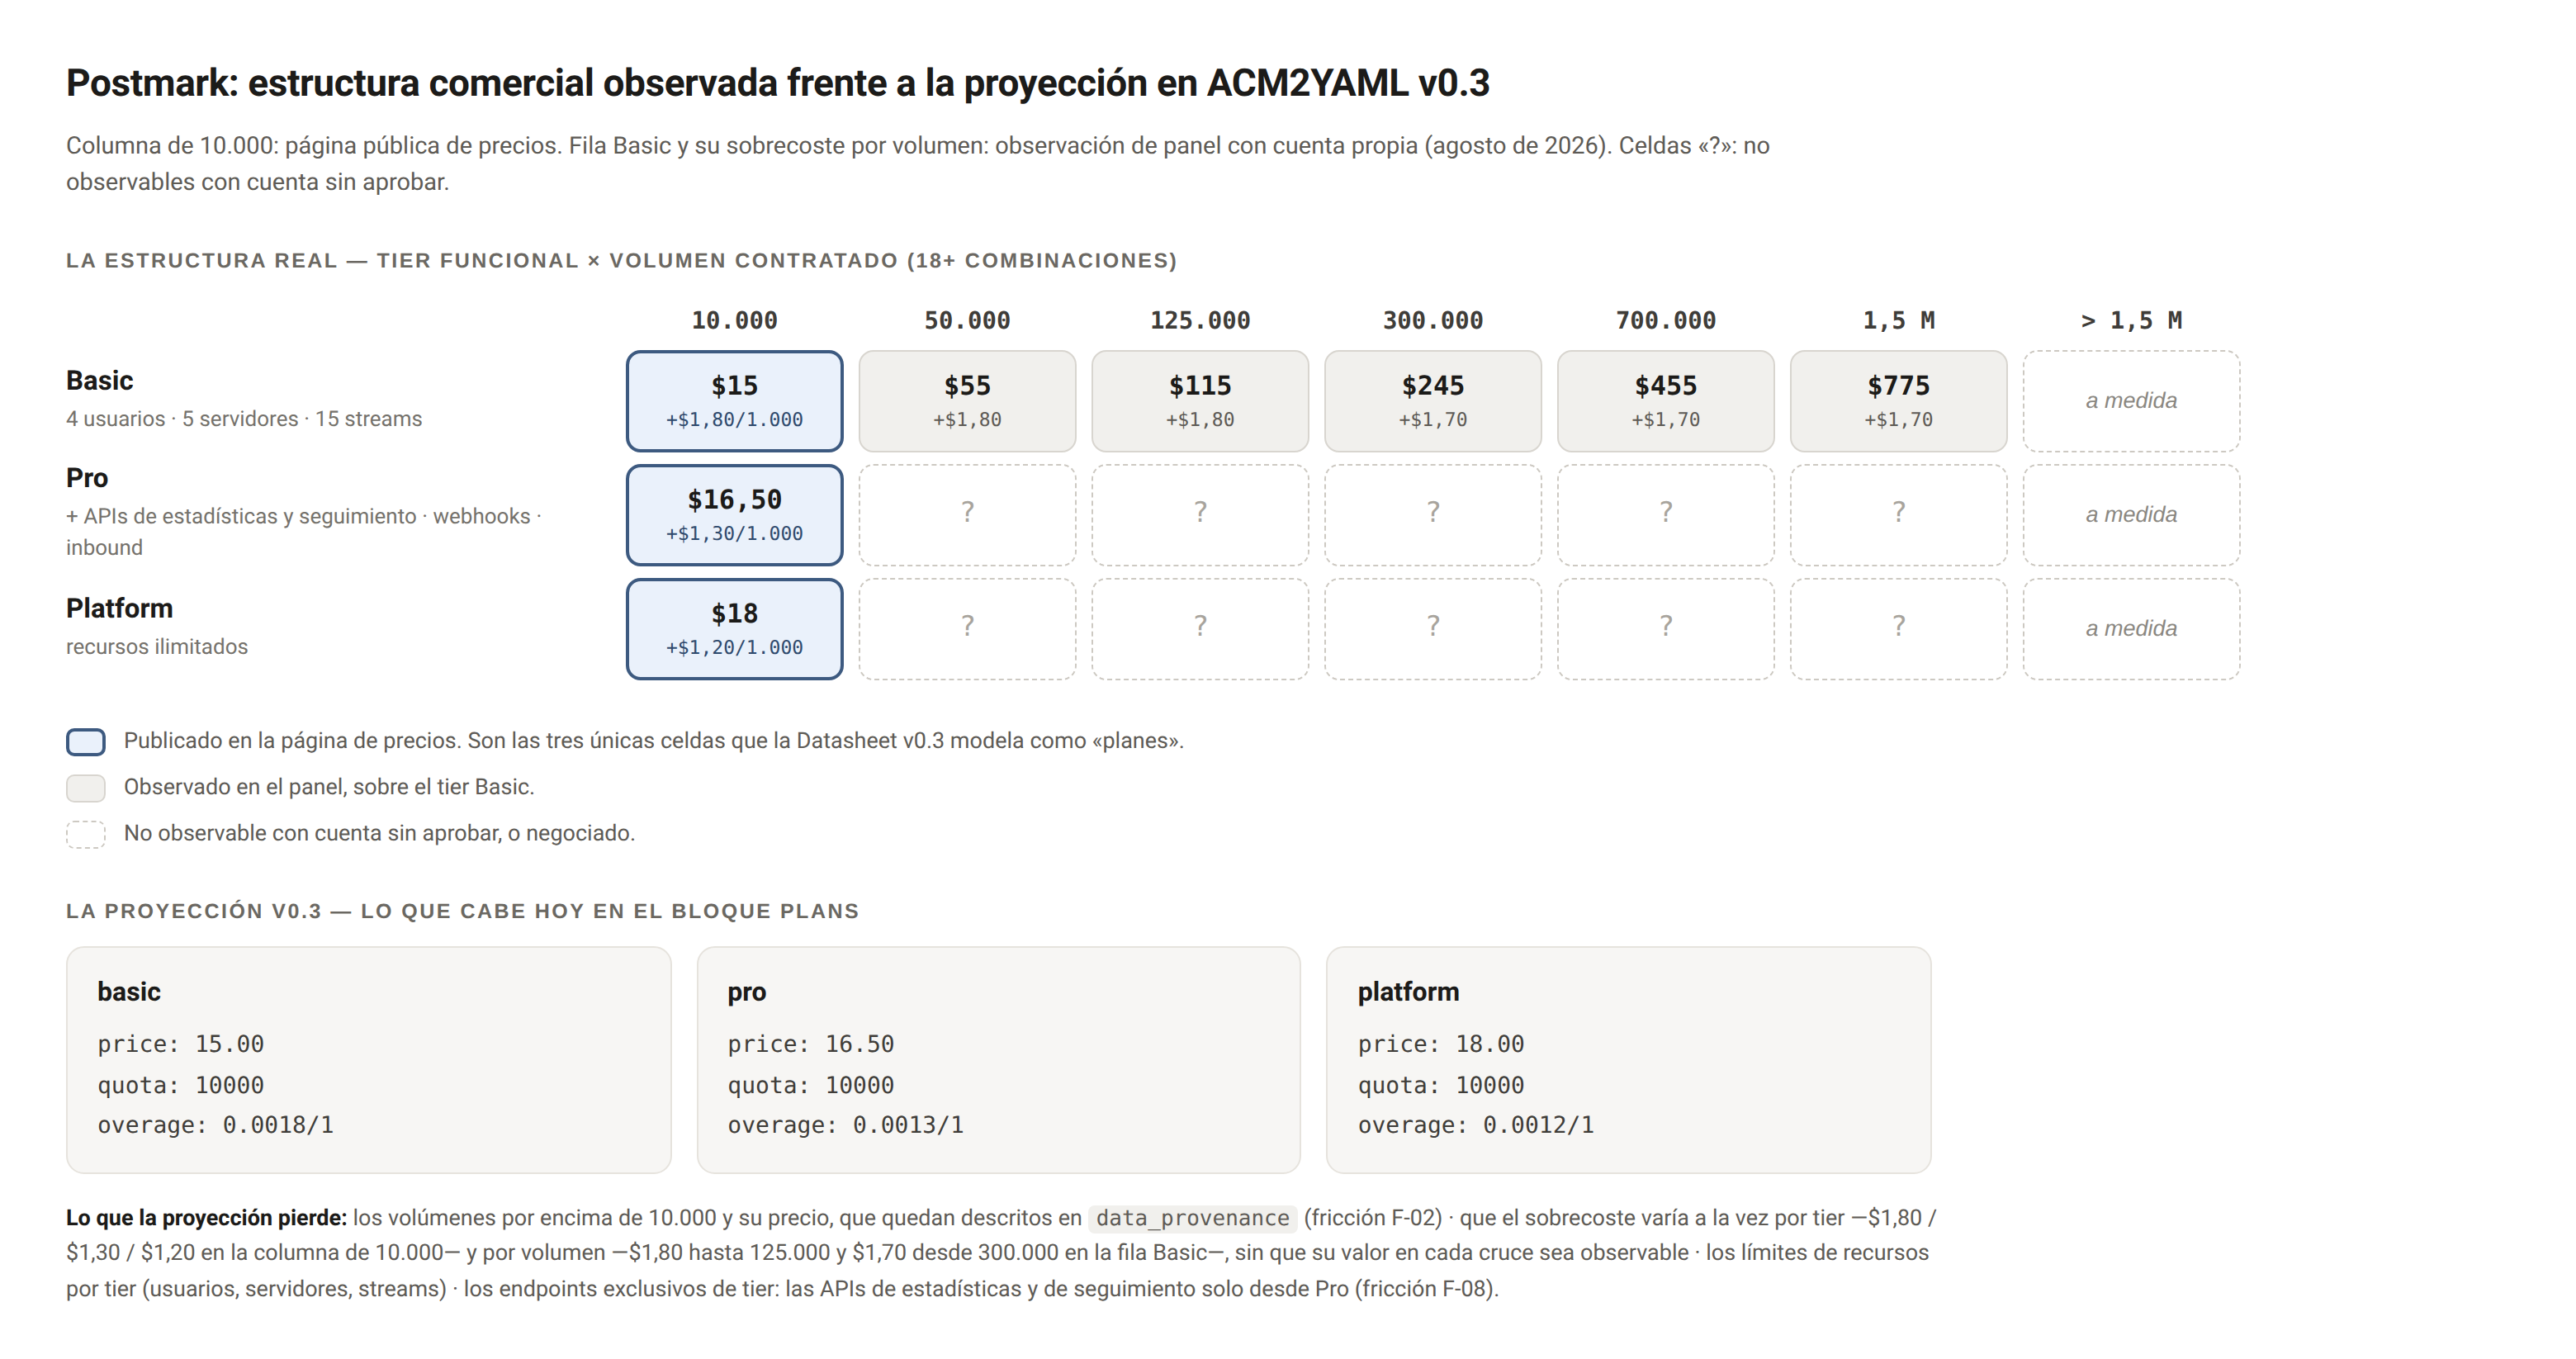
\includegraphics[width=\textwidth]{fig/tier_volumen_postmark.png}
\caption[Estructura comercial de Postmark frente a su proyección en el bloque \texttt{plans}
de ACM2YAML v0.3]
{Estructura comercial de Postmark (\textit{tier} funcional
$\times$ volumen contratado) frente a la proyección representable en el
bloque \texttt{plans} de ACM2YAML v0.3. La columna de 10.000 procede de
la página de precios \citep{postmarkpricing}. La fila Basic y su
sobrecoste por volumen proceden de la observación de panel con cuenta propia.
Las celdas sin valor no son observables con una cuenta sin aprobar.
Elaboración propia (agosto de 2026).}
\label{fig:tiervolumen}
\end{figure}

Tercero, el sondeo empírico desmintió a la documentación en un dato que
condiciona el análisis de capacidad. La referencia de la API declara un
máximo de cincuenta destinatarios \textit{por campo} (To, Cc y Cco), lo
que sugiere hasta ciento cincuenta por mensaje. Las peticiones de sondeo
demostraron que el límite real es de \textbf{cincuenta destinatarios
totales por mensaje}: cincuenta se acepta en cualquier reparto entre
campos y cincuenta y uno se rechaza en todos, y el propio mensaje de
error lo confirma de forma literal. La discrepancia queda registrada con
ambas citas. El sondeo del 7 de septiembre acotó después el factor de consumo por petición del envío por lotes: hasta quinientos mensajes por llamada, con cincuenta destinatarios cada uno (Apartado~\ref{subsec:hallazgos:postmark}).

Y cuarto, el piloto dejó un inventario de ocho elementos no soportados documentados
entre el dominio y el esquema, que la Tabla~\ref{tab:fricciones} sintetiza
junto con su estado en el marco de recurrencia. Ninguno de ellos impide la
conformidad del catálogo.
Todos eran candidatos a fundamentar las extensiones de la contribución C-02 hasta que el resto del dominio confirmara (o desmintiera) su generalidad.
La Tabla~\ref{tab:recurrencia} recoge el veredicto de cada uno sobre las ocho APIs.

\begin{table}[H]
\centering
\small
\begin{tabular}{|l|p{8.6cm}|l|}
\hline
\textbf{Id} & \textbf{Elemento no soportado por ACM2YAML v0.3} & \textbf{Estado} \\
\hline
F-01 & Un \textit{rate} que existe contractualmente pero sin valor
publicado: el bloque vacío se confunde con ``sin límite'' & candidato \\
\hline
F-02 & Cuotas por volumen contratado, con sobrecoste dependiente a la vez
del volumen y del \textit{tier}, y tramo superior negociado & candidato \\
\hline
F-03 & Factor de consumo multiplicativo (mensajes $\times$
destinatarios) que una terna única no puede expresar & candidato \\
\hline
F-04 & Restricciones declaradas que el proveedor admite no aplicar o que
la respuesta a la petición no refleja & discusión \\
\hline
F-05 & La dimensión \textit{Results Per Request} existe documentada en el
dominio y v0.3 no la serializa & candidato \\
\hline
F-06 & Un \textit{workload} acotado por otra métrica (bytes de
\textit{payload}, tras codificación) y no por un entero & candidato \\
\hline
F-07 & \textit{Add-ons} que modifican dimensiones de capacidad,
condicionados a volumen y a \textit{tier} & candidato \\
\hline
F-08 & El ``plan'' real es \textit{tier} $\times$ volumen, con superficie
de API dependiente del \textit{tier} & candidato \\
\hline
\end{tabular}
\caption{Elementos no soportados documentados en el piloto. Su promoción requiere
recurrencia en al menos dos APIs del dominio, o una sola con la
consecuencia ejecutada sobre el consumidor de referencia
(Sección~\ref{sec:propuesta:conformidad}).}
\label{tab:fricciones}
\end{table}

El piloto cumple así las dos funciones que se le pedían. Ha calibrado la
mecánica del ciclo antes de escalarlo al dominio completo.
Y ha mostrado que el método produce a la vez lo que este trabajo persigue: Datasheets conformes sin extender el esquema y conocimiento fundamentado sobre los límites del modelo que las define.
La verificación por uso del Capítulo~\ref{cap:evolucion} mide si el motor de referencia puede consumirlas, y ninguna de las ocho resulta plenamente consumible por PRIME4API (Tabla~\ref{tab:verificacion}).
Fija además el formato de
presentación del catálogo. Cada API se expondrá como aquí (caracterización
breve, lectura resumida en tabla con su semáforo, huecos documentales y
elementos no soportados nuevos o recurrentes respecto al inventario vigente), con la
explicación del método ya dada por este capítulo, de modo que los
epígrafes sucesivos resulten más breves, uniformes y comparables. Los
capítulos siguientes aplican este ciclo al resto del catálogo y explotan
sus resultados.

\section{Respuesta a la pregunta de investigación}
\label{sec:propuesta:respuesta}

La RQ1 pregunta qué APIs de correo deben incluirse en un análisis representativo del dominio, y bajo qué criterios reproducibles.
La primera mitad se responde con una condición: el conjunto debe cubrir las cuatro formas de cobro del primer criterio, y sus APIs deben diferir en los rasgos de límites que pide el cuarto.
En la ventana de toma de datos (Apartado~\ref{sec:propuesta:ventana}), las ocho APIs de la Tabla~\ref{tab:propuesta:rq1} forman un conjunto que la cumple.
La condición fija qué debe cubrir el conjunto, y otro que cubriera lo mismo también la cumpliría.
La segunda mitad la responde el protocolo de la Sección~\ref{sec:propuesta:seleccion}, y el Anexo~\ref{anx:uso-ia} registra la consulta.

\begin{table}[H]\centering\small
\begin{tabular}{|p{2.3cm}|p{1.6cm}|p{3.8cm}|p{5.6cm}|}
\hline
\raggedright\textbf{API} & \raggedright\textbf{Fuente} & \raggedright\textbf{Forma de cobro según la respuesta} & \raggedright\textbf{Lo que registró la construcción} \tabularnewline
\hline
\raggedright Postmark & \raggedright Piloto & \raggedright Planes por volumen mensual & \raggedright El plan real es \textit{tier} $\times$ volumen contratado (Sección~\ref{sec:propuesta:piloto}) \tabularnewline
\hline
\raggedright Resend & \raggedright Segunda & \raggedright Planes por volumen con caudal negociado no publicado & \raggedright Planes por volumen mensual, con Enterprise sin precio, volumen ni \textit{rate} publicados y Free con 100 correos al día y 3.000 al mes (Apartado~\ref{subsec:hallazgos:resend}) \tabularnewline
\hline
\raggedright SendGrid & \raggedright Segunda & \raggedright Planes por volumen mensual & \raggedright Planes por volumen mensual, cuyo sobrecoste tiene techo desde el 26 de marzo de 2026 (Apartado~\ref{subsec:hallazgos:sendgrid}) \tabularnewline
\hline
\raggedright MailerSend & \raggedright Segunda & \raggedright Planes por volumen mensual & \raggedright Planes por volumen mensual, y es la única con cuota diaria de peticiones junto a la mensual de correos (Apartado~\ref{subsec:hallazgos:mailersend}) \tabularnewline
\hline
\raggedright Brevo & \raggedright Tercera & \raggedright Planes por volumen con límite diario adicional & \raggedright Límite de 300 correos al día en Free y volumen mensual en los planes de pago (Apartado~\ref{subsec:hallazgos:brevo}) \tabularnewline
\hline
\raggedright Amazon SES & \raggedright Tercera & \raggedright Pago por uso puro & \raggedright Pago sin plan y, desde el 21 de julio de 2026, planes (Apartado~\ref{subsec:hallazgos:ses}) \tabularnewline
\hline
\raggedright Mailgun & \raggedright Tercera & \raggedright Planes por volumen mensual & \raggedright Planes por volumen mensual, sin umbral en la documentación de la API y con un único caudal publicado para la API REST, en las preguntas frecuentes y por IP de cliente (Apartado~\ref{subsec:hallazgos:mailgun}) \tabularnewline
\hline
\raggedright Mailchimp Transactional & \raggedright Tercera & \raggedright Añadido de otro producto, por bloques & \raggedright Complemento de los planes Standard y Premium o del mensual heredado, sin planes con nombre, en bloques de 25.000 correos (Apartado~\ref{subsec:hallazgos:mailchimp}) \tabularnewline
\hline\end{tabular}
\caption{Las ocho APIs del catálogo. La segunda columna indica la fuente de inclusión (Apartado~\ref{sec:propuesta:fuentes}). La tercera reproduce la clasificación de la respuesta a la consulta (Anexo~\ref{anx:uso-ia}). La cuarta dice qué forma de cobro encontró la construcción en la ventana de toma de datos y añade un rasgo de la API.}
\label{tab:propuesta:rq1}\end{table}

La consulta pedía cubrir las cuatro formas de cobro, y la construcción las encontró todas en el catálogo.
También corrigió tres afirmaciones de la respuesta.
La respuesta describía Amazon SES sin planes, y el proveedor los tenía desde el 21 de julio de 2026, antes de la consulta.
Atribuía a Mailgun \textit{rates} publicados por endpoint, y la documentación de su API no publica ningún umbral.
El único caudal que el proveedor publica para su API REST está en sus preguntas frecuentes, acotado a una IP de cliente.
Presentaba la combinación de cuota diaria y mensual como aportación de Brevo, y esa combinación ya estaba en el plan Free de Resend.
La primera y la tercera corrección muestran además que las formas de cobro no son excluyentes.
Ninguna de las tres correcciones activa la regla de reemplazo, que solo depende de la trazabilidad (Apartado~\ref{sec:propuesta:reserva}).

El Capítulo~\ref{cap:hallazgos} muestra qué aporta el conjunto frente a sus cuatro primeras APIs.
Postmark, Resend, SendGrid y MailerSend tenían planes con cuota mensual.
Todas tenían además sobrecoste decreciente y tope de destinatarios.
Amazon SES, Brevo y Mailchimp Transactional, que la respuesta justificó por su forma de cobro, carecen de al menos uno de esos rasgos.
Mailgun, que según la respuesta comparte forma de cobro con Postmark, SendGrid y MailerSend, es la única del catálogo que contesta por escrito sobre la concurrencia de su API REST.
La Sección~\ref{sec:hallazgos:limites-rates} recoge seis afirmaciones que solo son visibles con las ocho APIs.
En esta memoria, un análisis del dominio es representativo cuando cumple la condición con que se abre esta sección, fijada con los criterios antes de la consulta.
La cuota de mercado de cada API no se midió y no entra en esa condición.

Este cierre de la RQ1 tiene limitaciones conocidas, y las primeras están en las fuentes.
La primera fuente no se ejecutó.
Postmark entró como piloto del método y no por una de las tres fuentes.
Los cinco criterios solo decidieron cuatro de las ocho APIs: la consulta clasificó las otras cuatro por su forma de cobro, sin evaluarlas.
El prompt ya fijaba un catálogo de ocho APIs, y ese tamaño no se deriva de la cobertura.

Otras están en los criterios.
La respuesta da por cumplidos dos de ellos sin aportar evidencia: la documentación pública del segundo y la adopción real del tercero.
La documentación pública no cubrió todos los límites, y la construcción necesitó el panel con cuenta propia para algunos, como la cuota mensual del plan Free de Mailgun.
Las cuatro formas de cobro se fijaron en el primer criterio antes de la consulta, sin un censo del mercado ni una lista cerrada de candidatas.
Las diferencias en los límites que muestra el Capítulo~\ref{cap:hallazgos} se observaron después, sobre las ocho APIs, y describen la muestra sin garantizar que esté completa.
Mailchimp Transactional fue una de las dos últimas en construirse.
Resultó ser la única API sin planes y la única sin tope de destinatarios.
Una novena API podría añadir otro rasgo.

La regla de reemplazo es ordinal, y de haberse aplicado no garantizaba conservar la forma de cobro de la API sustituida.
Si hubiera salido Amazon SES, habría entrado Mailjet, y el catálogo habría perdido la única API que la respuesta clasificó como pago por uso puro.

Las últimas están en la consulta, cuya respuesta no se repite con garantía.
La consulta se hizo en la sesión de trabajo del proyecto, y la respuesta cita dos decisiones previas que el prompt no recoge.
Un tercero con el mismo prompt y sin ese contexto puede obtener otra respuesta.
El registro tampoco recoge cuántas veces se lanzó la consulta.
El protocolo permite a ese tercero contrastar la respuesta que obtenga con los criterios y con lo que registre la construcción, como hace esta sección con la consulta del 1 de septiembre de 2026.
